% CHAPTER 1
\setcounter{chapter}{0}
\chapter{Introduction}
\thispagestyle{plain}


%Box with Learning objectives should be at the beginning of each chapter

\begin{corollary}

	\hspace*{10mm}
	
	\vspace{5mm} %for optical corrections
	% optionaler Text	
	
	\begin{itemize}
			\item Introduction
			\item Speech Production
			\item Source Filter Model
			\item Hearing
	\end{itemize}
\end{corollary}

\clearpage

%Einf�hrung in das Kapitel



% CHAPTER 1 LESSON 1
\clearpage
\section{Introduction}
\label{Introduction}



%Einf�hrung in das Kapitel

Humans have evolved with the unique ability of manipulating their lungs and vocal tracts to convey information to each other.  Although other animals produce and react to inter psecial vocalizations, humans have the amazing unique ability to produce and interpret these sounds, allowing them to impart knowledge about complex emotional states and information about the world we live in. The importance of speech to being human can be seen in the development of blind and deaf children.  Although both cases face hardships associated with their handicap, deaf children, denied of proper therapy, face challenges in social maturation that are not seen in blind children.

Because speech is such an essential human trait, the biological processes that are responsible for producing and perceiving it are the subject of continuous scientific research and development.  The microphone, in a general way, performs the same function as our inner ear, converting vibrations into a series of voltage fluctuations.  Modern computers can even mimic basic cognitive functions of the brain.

The purpose of this class is to study some underlying processes involved in speech production and perception.  This a priori knowledge can then be used to develop algorithms that allow us to digitally manipulate speech to benefit those suffering from diseases affecting speech production or perception.  It also allows us to communicate more.











% CHAPTER 1 LESSON 2
\clearpage
\section{Speech Production}
\label{Speech Production}

Speech production begins with the lungs. The lungs produce the airflow and therefore the energy required to produce speech. This energy then flows through the larynx where the vocal chords are located.  The vocal chords can then begin to vibrate to produce a voiced speech sound or not vibrate to produce an unvoiced speech sound.  This excitation then passes through the vocal tract whose shape can be modified through changes of the tongue, lips, jaw, etc. Each shape corresponds to a different resonance, almost like filling a glass with with different levels of beer to produce different tones.  It is these resonances that produce the different speech sounds that we can then understand.\\
\\
Figure 1, depicts the different parts of the vocal tract that are involved in producing speech. The main two sections are the oral cavity and the nasal cavity. These are separated by a sort of switch called the valluum. The tongue and lips also have important functions in changing the volume of the vocal tract and therefore producing different vocal sounds.\\

\begin{wrapfigure}{r}{0pt}
    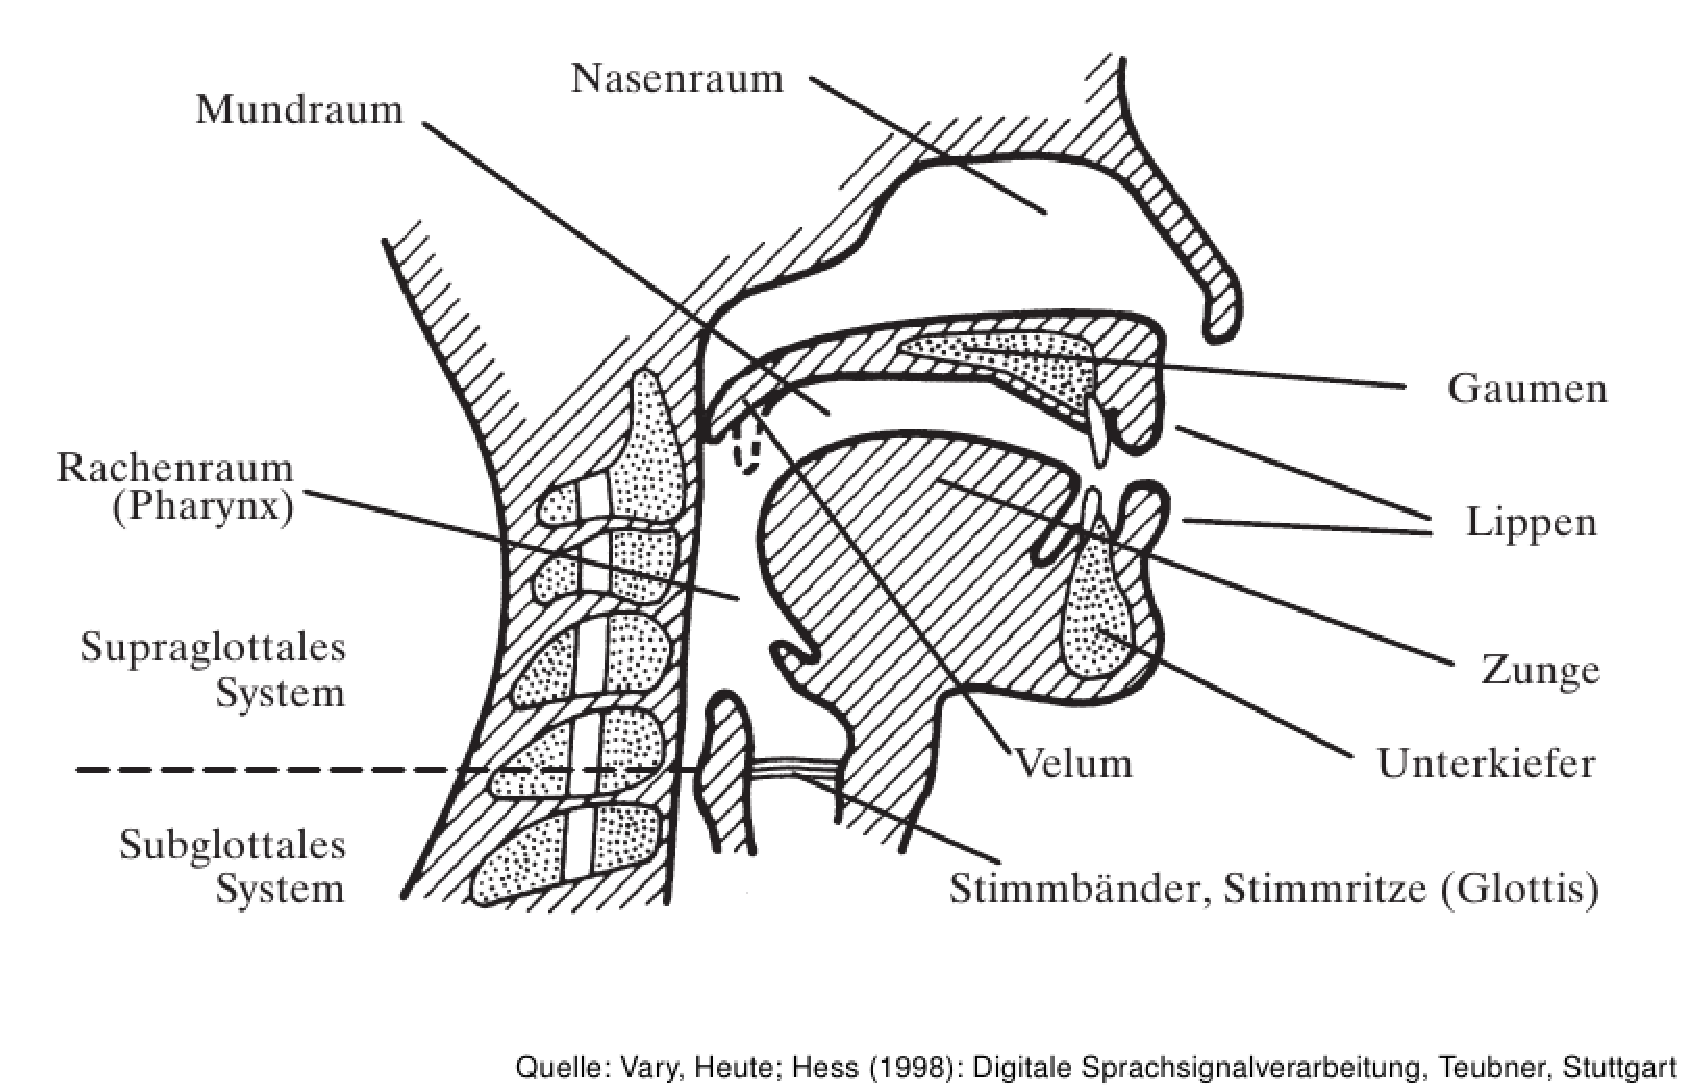
\includegraphics[width=0.7\textwidth]{Pictures/Chapter1_Lesson2/vokaltrakt-eps-converted-to.pdf}
    \caption{The vocal tract.}
\end{wrapfigure}

There are many speech sounds that we can produce and these sounds change for different languages. Probably the most obvious distinction that we can make between all of these vocal sounds is to separate them into voiced and unvoiced. Voiced speech sounds are those produced when our vocal chords vibrate. The best examples are the vowels.  These are sounds where the excitation signals are a periodic vibration of the vocal chords.  There are also unvoiced sounds. These are sounds where the glottus is not vibrating.  These are sounds such as the fricative  /sh/.  Plosives are also unvoiced speech sounds where there is a  complete constriction of the vocal tract and then a sudden opening such as /k/,/p/,/t/.  There are also sounds that are mixture of the two types of excitation such as /v/. \\
\\
Figure 2 shows how these different speech sounds look in the time domain. It was said that a voiced speech sound has a periodic excitation.  This can be seen in the periodic structure in the time domain plot.  The distance between two peaks in the plot is called the fundamental period, or the difference in time between the opening of the glottus. Fig 2b depicts an unvoiced speech signal.  Because there is no periodic excitation of the glottus, the excitation signal is more random in nature. This can be seen by the amount of zero crossings in the time domain plot.  Fig 2c shows a transition between two speech signals.\\

\begin{wrapfigure}{l}{0pt}
    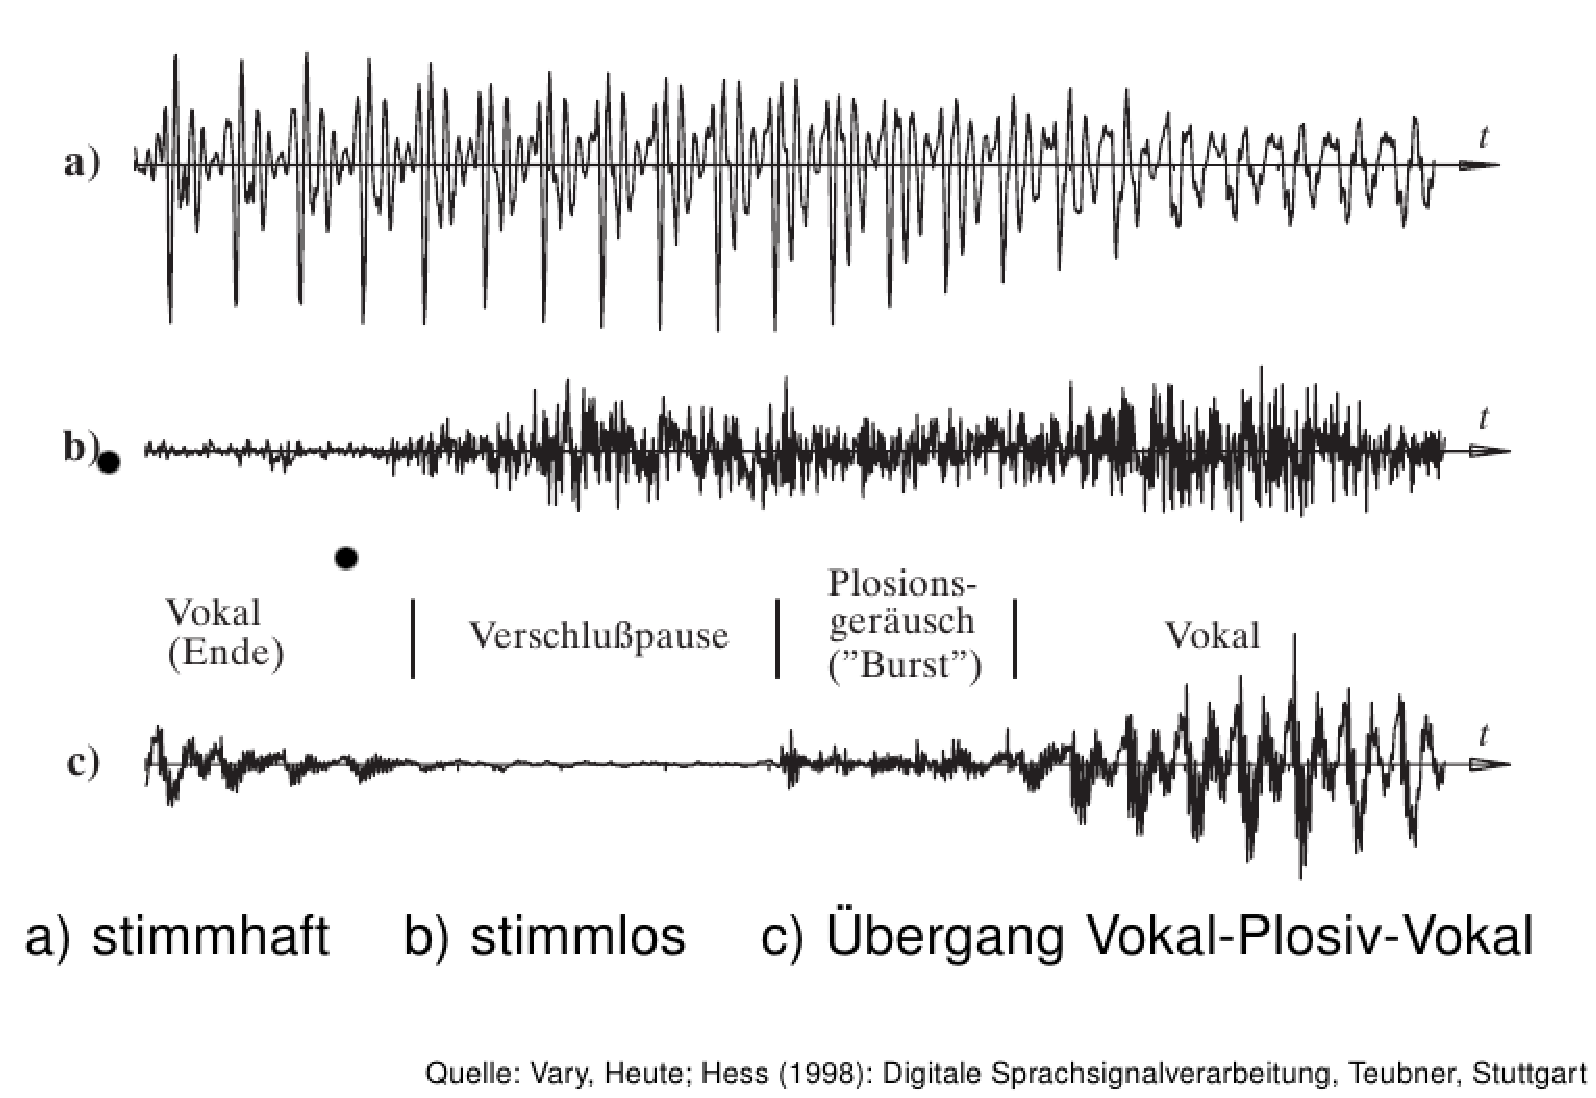
\includegraphics[width=0.7\textwidth]{Pictures/Chapter1_Lesson2/sprachlaute-eps-converted-to.pdf}
    \caption{Time domain signals of voiced and unvoiced speech.}
\end{wrapfigure}

Speech sounds convey meaning and because some of these sounds are different, however still convey the same meaning, there is a system to classify them. A phone is defined as the smallest speech segment with distinct physical or perceptual properties. To call a speech sound a phone is to say that there are no other segments of speech that are the same as that particular segment of speech.  Then there are phonemes.  These are the smallest segments of speech that can change the meaning of a word.  The phoneme consists of a set of phones, so phones are actually different realizations of a phoneme. All of the phones that belong to one phoneme are called allophones. One allophone is one phone of the many that constitute a phoneme. One phoneme can consist of many allophones.  For example, if you take the words ''kiss'' and ''kill'', they have very different meanings, however the difference is only in the phoneme at the end.  This is different with the words  ''cat'',''kit'', ''school'', ''skill''.  These all contain the phoneme /k/ but are pronounced differently due to the different vowel transitions and would, therefore, all be classified as different phones of the same phoneme /k/.\\
\\
Natural human languages have between 10 and 80 phonemes. These can be characterized by the way in which they are articulated, whether they are voiced or unvoiced, and in which place they are articulated.  Place of articulation is basically saying where the tongue is placed in order to produce the speech sound. The different parts of the vocal tract can be used to generate the different phonemes and are also differ across cultures.  The Americans use quite a bit of retroflex, rolling the tongue backwards to create a rolled  ''r' sound. Germans tend to use a glottal stop to distinguish between ''verreisen'' and ''vereisen''. There is a phonetic alphabet that can be used to describe all languages. Fig 3 shows this phonetic alphabet distinguished by place and type of articulation.\\

\begin{wrapfigure}{l}{0pt}
    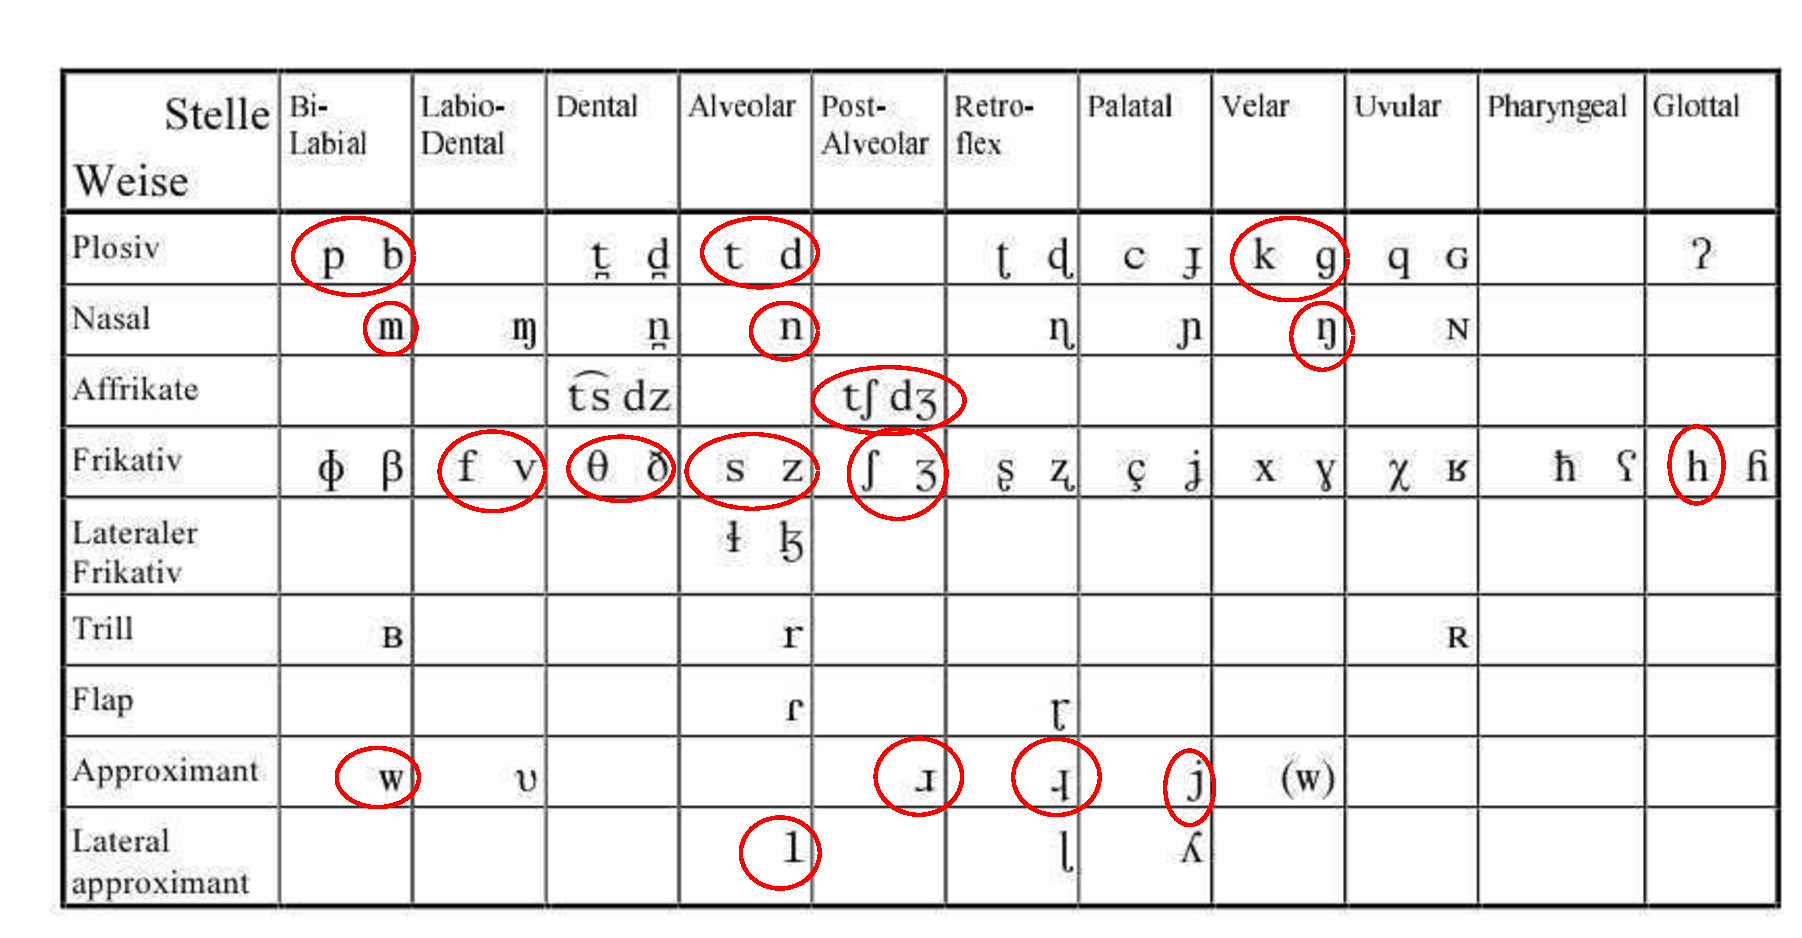
\includegraphics[width=0.7\textwidth]{Pictures/Chapter1_Lesson2/intPhonAlphabet_konsonanten_english2-eps-converted-to.pdf}
    \caption{The phonetic alphabet}
\end{wrapfigure}

Vowels can be distinguished by the position of the tongue in the oral cavity when they are generated.  These are called the cardinal vowels. As with the phonetic alphabet, we are looking for a language independent description. This is done by mapping the position of the tongue in two dimensions, Front to back and high to low, to the vowel sound.  This mapping can then be used to order the corresponding phonemes.  These are called the primary vowels as opposed to the secondary cardinal vowels which are less common and more difficult to say. On one axis, there is the positioning of the tongue from back to front, and then a different axis for the opening of the mouth. It is important to note that the secondary vowels are produced with open lips.\\

Co-articulation is a term used to describe the fact that we produce the same phonemes differently dependent on the content.  This is basically due to the fact that we cannot change our vocal tracts instantly, but there will always be a smooth transition of the tongue from one position to the next.  For instance when you say ''hen'',  it is usually an aveolar sound where the tongue is placed behind the front teeth. However if you say tenth, the /n/ is followed by a /th/, a more dental sound. Therefore, the /n/ will also be pronounced more dentally.  \\

Prosody is another important characteristic of speech.  It is defined as the rhythm, stress, and intonation of speech.  Mostly when people speak of prosody, they speak of the intonation of speech, the melody of the sentence that is said. However, the concept of prosody also encompasses the rhythm and the stress of a speech utterance. Prosody also carries information. It could be the difference between a question and a statement. If we ask a question, we usually raise the fundamental frequency at the end of the sentence.  We also use it to put emphasis on certain words. ''Put the GREEN ball on the table''.  ''Put the green BALL on the table''.  It also carries information about the emotional state of the speaker. For instance, if I yell, then this will usually have a different meaning than if I whisper.  


% CHAPTER 1 LESSON 3
\clearpage
\section{Source Filter Model}
\label{Source Filter Model}

The previous lesson introduced the method by which we produce speech. The lungs produce energy, in the form of airflow, that passes through the larynx where either oscillating vocal chords produce voiced speech or the airflow simply passes through to produce unvoiced speech.  This energy then passes through vocal tract, where the current positioning of the jaw, lips, tongue, etc. affect the shape and therefore the speech sound that is uttered.  This process can be modeled by a source filter model.  This assumes that we have a source, the airflow after it passes through the larynx, and then a filter which is defined by the resonance frequencies of the vocal tract. In this model, we assume that these two are independent. This is a very critical assumption and important to understand and would require, for example, that the resonances of the vocal tract are independent of the fundamental frequency of the excitation. The ultimate goal is to model this process mathematically and for this we have to understand what is really going on in the process. \\

\begin{wrapfigure}{l}{0pt}
    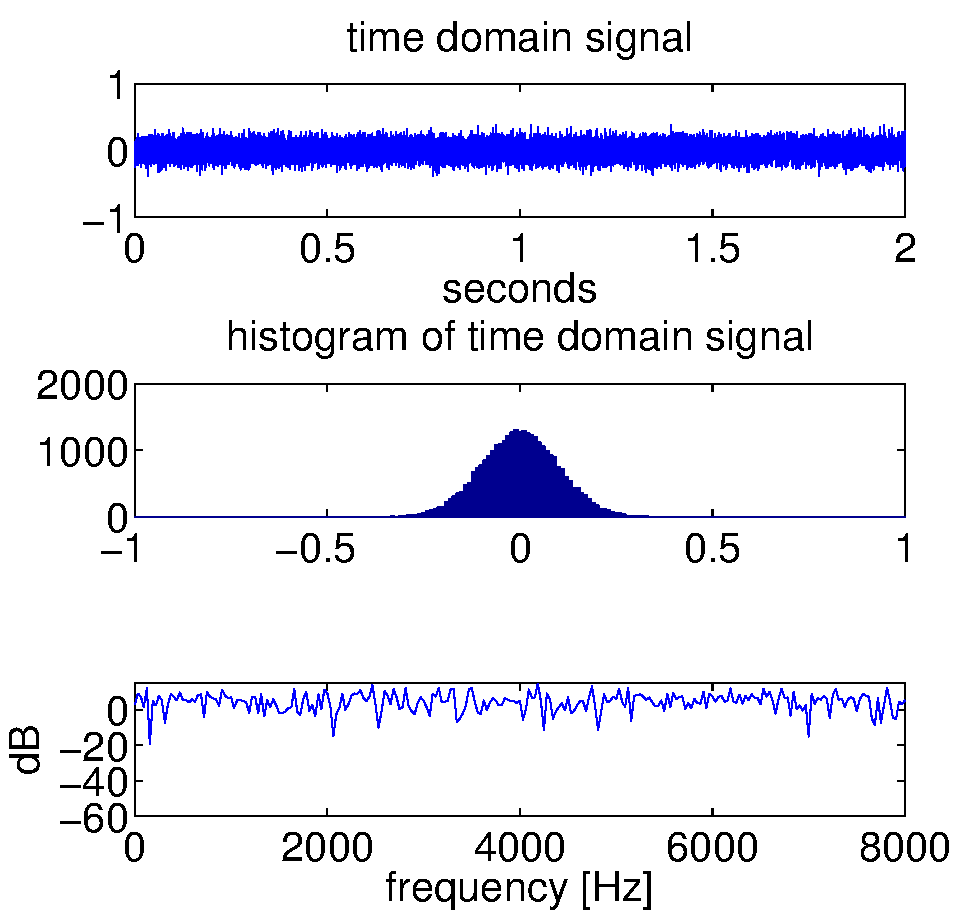
\includegraphics[width=0.5\textwidth]{Pictures/Chapter1_Lesson3/gaussianNoise-eps-converted-to.pdf}
    \caption{Statistics of white Gaussian noise.}
    \label{gaussNoise}
\end{wrapfigure}

The excitation signal for a unvoiced sounds is described  by turbulent airflow passing through the glottis. This can be modeled by using white Gaussian noise. The top of fig \ref{gaussNoise} depicts the time domain signal of white Gaussian noise. It is Gaussian noise, because a histogram of the samples in the signal will produce a Gaussian distribution. As can be seen in the histogram, there are more values close to zero than there are towards the edges. It is white noise, because a Fourier transform of the signal produces a flat spectrum.  The term ''white'' refers to a flat spectrum because in optics, white light as composed of an equal amount of energies of all frequencies, whereas light that has more energy in lower frequencies would be red.\\



For a voiced excitation, the vocal chords open and close periodically. If we look at the glottal flow behind the larynx, what is observed is a periodic form. First, we start with closed vocal chords, a closed glottis. Next, as we produce energy with our lungs, we push air and the glottis opens because there is an increased pressure that builds up at the base. As the glottis opens, the pressurized air can now escape and the thus, the airflow increases and by Bernoulli's principle, the pressure decreases. Because the vocal chords are under tension, this decrease in pressure allows them to snap shut to begin the process again. This is the mechanism behind voiced excitation. \\

\begin{wrapfigure}{l}{0pt}
    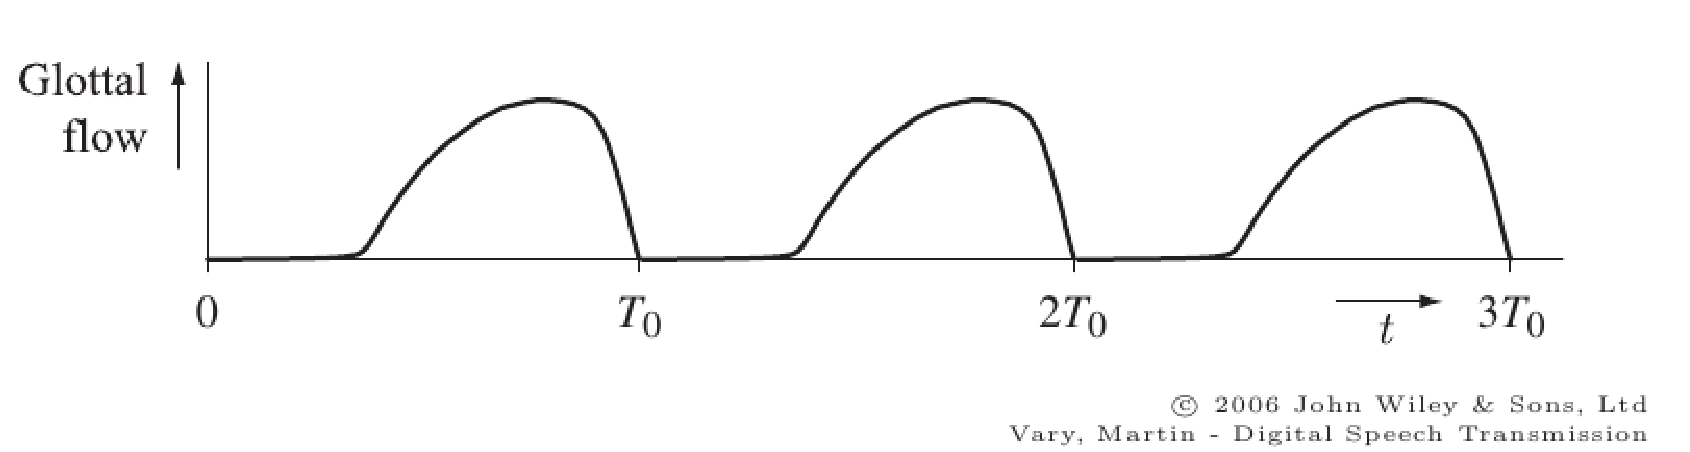
\includegraphics[width=0.5\textwidth]{Pictures/Chapter1_Lesson3/glottalFlow-eps-converted-to.pdf}
    \caption{Glottal flow over time}
    \label{glotFlow}
\end{wrapfigure}

 The two forms of excitation can now be described in a simple model. In the unvoiced case,  a noise generator can be used to produce the excitation energy.  For voiced speech, a pulse train in the time domain can be used with a peak to peak distance of the fundamental period, \begin{math}T_0\end{math} This will model the opening and closing of the glottis.  It is then necessary to have a switch that chooses between the two forms of excitation and some form of detector that can determine which excitation is present in the current speech signal.  There are also mixed excitation sounds, so one could also imagine there being a weighted summation of the two excitation signals, so we could have something that's a little more complicated like a weited summation to produce mixed excitation signals. \\

The next step is to model the vocal tract as a filter through which the excitation signal passes. The vocal tract can be thought of as a filter because it will have certain resonance frequencies similar to the resonances of a tube. In fact, the vocal tract can be simplified by using a tube model in which there is one input and two outputs, the lips and the nose. This can be seen in fig \ref{tubeModel}, where the tube on the bottom represents the oral cavity with another tube on top representing the nasal cavity.  The tubes will be separated by a switch that models the vallum.  Each tube will have its own resonance.  By modifying the shape of the tube, different resonances would be produced thus producing different speech sounds .\\

\begin{wrapfigure}{l}{0pt}
    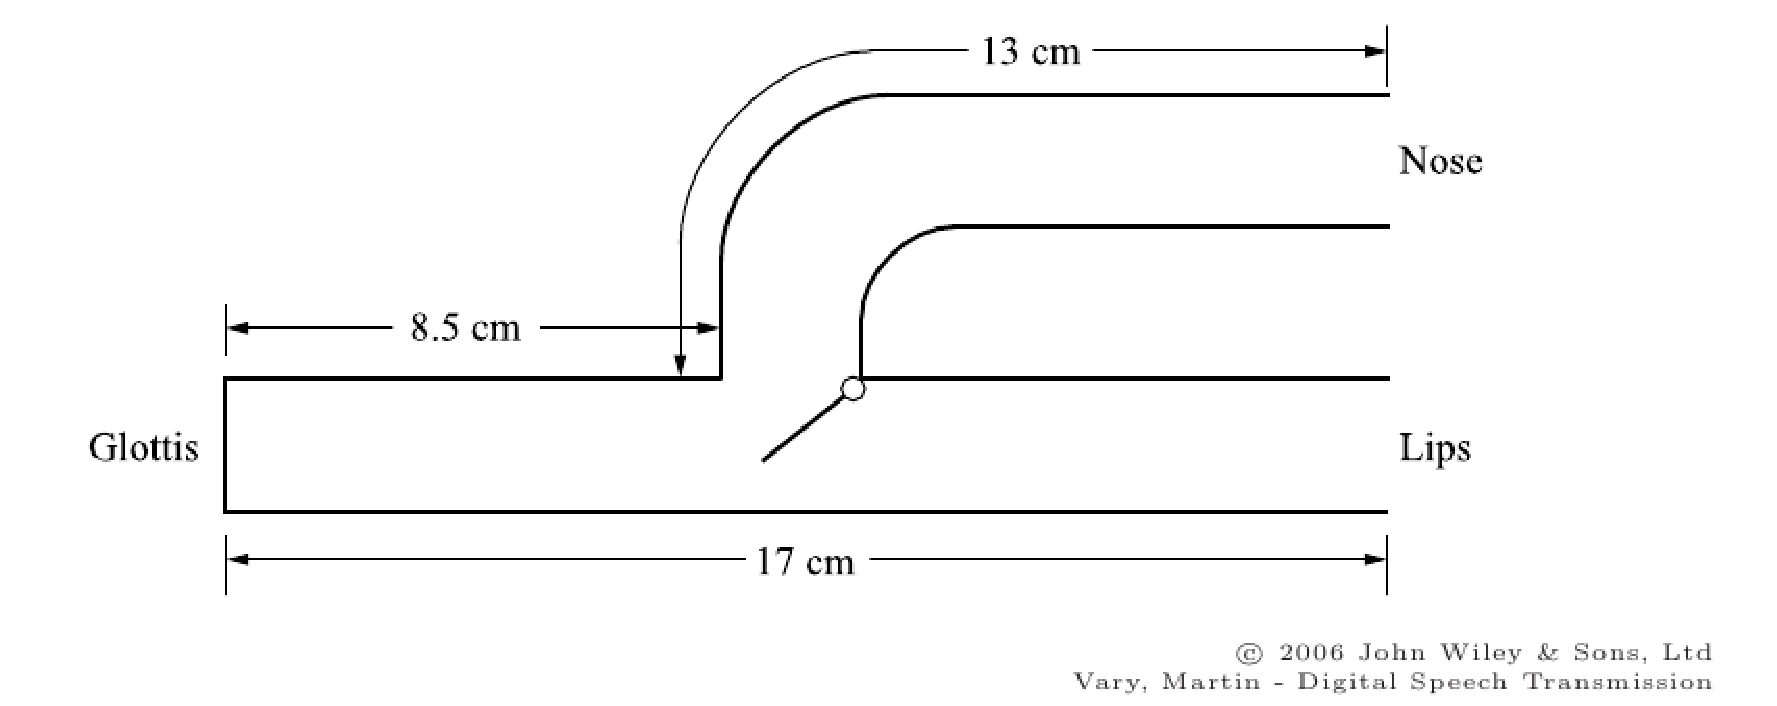
\includegraphics[width=0.7\textwidth]{Pictures/Chapter1_Lesson3/vocalTractSimple1-eps-converted-to.pdf}
    \caption{Simplified model of the vocal tract.}
    \label{tubeModel}
\end{wrapfigure}

From a signal processing view, the vocal tract filters the excitation signal to produce a speech sound. Mathematically speaking, this is represented by a convolution in the time domain and a multiplication in the frequency domain. The vocal tract can therefore be thought of as a transfer function. The spectrum of this transfer function would contain certain resonances. This can be seen in fig \ref{transFunc}. In signal processing, these are called formants, the resonances of the vocal tract. Formants contain important information because they decide what speech sound is being produced.  When the spectra of the excitation signal and the vocal tract transfer function are multiplied, what is seen is the result of what would happen if we did a frequency analysis of a recorded speech sound. The influence of the excitation signal and the vocal tract can both be seen in the final signal. It is very important to understand that these are two independent signals in our model. Notice that at the bottom of fig \ref{transFunc}, the formant peak is not seen. It lies between the two peaks of the harmonics because the final signal is an almost sampled version of the vocal tract function. Babies are very skilled at aligning the fundamental frequency with the formant, because this is when they scream the loudest! If the harmonics are between the peak of the formants, the energy in the final signal would be lower as opposed to the harmonic being aligned with the formant.  The peaks of the formants are given by the multiple peaks seen  in the transfer function, whereas the fundamental frequency is given by the first peak of the fine structure or the distance between two neighboring peaks.\\

\begin{wrapfigure}{l}{0pt}
    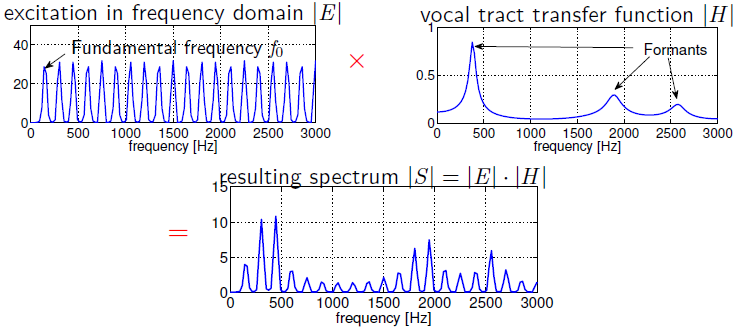
\includegraphics[width=0.7\textwidth]{Pictures/Chapter1_Lesson3/Transferfunc.png}
    \caption{Transfer function of the vocal tract.}
     \label{transFunc}
\end{wrapfigure}

Formant freq vs fundamental freq.  
Formants are imporatnt becasue they define the meaning of a speech sound.

We can then draw a formatn map with this information.  If we look at the map, we can see a caertain area  where phonemens have their formants. How lare the area is depends on the database used to create it .

It is imporant to understand the difference between fundamental frequecny and formants.  The formants carry the meaning where as the fundamental frequency refers to the excitiation signal and carries no real meaning (only with respect to tintonation prosody)

So for simple model of speech production there are certain parameters taht we need to know.  We would need to know: voiced/unvoiced speech signal to switch our excitiation and for this one, we would need to know our fundamental period, and our voacl tract transfer function.


% CHAPTER 1 LESSON 4
\clearpage
\section{Hearing}
\label{Hearing}

The ear, ruglhly speaking consists of different parts, the outer ear, the middle ear and the inner ear. the outer ear consistrs of the pinna the ear canal and the ear drum and the middle ear consist of the jkahsfda stapus which work like a leather.  The inner ear consists of the cochlea which is where we perceive sound and is where the auditory nerve is attached. Sound aves travel through the ear canal and cause the ear drum to vibrate and we have this lever here so we transistion from the large area to the samall area and here we would have then the travelling wave travelling through the cochlea. Here we would have the basilarmembrane.

The intersting thing is that the basilar membrane does the frequency to place transformation meaning that we have a travelling wave that will have its peak at certain point in space, for instance if we have a tone a 3500hz then it would have its maximum at a certain point if we have a high frequency tone the maximum would closer to the base of the badilar membrane so the point where the stapus, while if we have lower frequenceies , the resonances will be toward the apex.  so the tip of the cochlea and thats very imporatn becasue it means that we also perceive sound in the frequency domain m,eaning that humans perform a frequency analysis of the signal . Thats also why this frequency analysis that we use is so natural for us because it is also how we perceive sound .

If we look a little closer, at a cut through the cochlea we will see these tubes that wind up.  The interesting part is the basilar mnembrance and the ortgan of corti  where we have the hair cells.  What happens is that there will be a travelöling wave that will cause this part to move against the tectortial membrnce so that we will have the movemnet of the hair cells and they will then fire through the auditopry nerve and then the brain will have a percepotion of sound .

SO this is the auditory sensation area for a normal hearing person, so we have acertain threashlod of hearing here we see the frequecny axis on a logarithmic scaling. So we can see that at lower frequencies, we need more energy to perceive sound than at higher frequencies up to a caertain order.  Frequencies below 20Hz we are not able to perceive, at least not throught the cohclea and also at higher frequencies, we have problems as we get older. At the top is the level of pain. If we hear a sound at a level higher than the line for an extenden period of time, we will start to have hearing damage. We can see that speech fills a certain range in the auditory senstaion area.   Interestingly, the area where all the formants are is also the area where our ear is most sensitive. Quite conveninet It means that our ear is optimized for speech perception. (or the other way around) We see taht music has a wider range in frequency.  If you listen to the radio we hear that it sounds difffernt but we can still understand everything that is being said, this is because we still transmit the important formants even though the music range is much wider.

So what happens if we are hearing impaired or if we experience a sernsory neural hearing loss? So what happens approximately, or simply speaking is that the level of pain approx dont change, while the threshlod of hearing is increased.  We then need to amplify soft sounds but if we would just linearly amplify the level of sounds, we would o that beyond the level of pain and thats why we need compression algorithm in hearing aids, so tha twe amplify soft sounds more than loud sounds.  This decreases the SNR and therefore requires some noise reducxtion to enhance the signal to our hearing aid. 

Its interesting to note that there are different types of hearing losses.  The conductivbe hearing loss is the one can be traeated more easily that a senorsneural hearing loss  because it means that the sound is not properly conducted by the outer ear or the middle ear. The bomes could stiffen The sound is still perceiveable, but attentuatoed which also means that you can also treat it rather well with a hearing aid by amplyfying the sound. Sensorineural hearing loss is for instance what we have with th age related hearing loss so we get older then our hair cells die. They can also die because of trauma for instance if you are in very noisy or loud environment or if there is a gunshot. This can dmage the hair cells and then there is nothing that we could do at this time.  This sensory neural hearing loss is often accompanied by tinnitus where when one doesnt hear well, instead they hear a ringing. And then what else happens is that soft sounds are too soft and loud sounds are too loud which basically measn that we have this reduced area in the auditory sensation map. Whats also problematic is that the sensory neural hearing loss goes along with a decrease in frequency resolution meaning thta even if you do a audtitory test, you can still preform well to some extent, but still you have trouble when you want to perceive speech in noise cause the frequency resolution of your auditory perception is decreased. And this means that we cannot so well distinguish between speech commands. And that means that we have a decreased speech understanding in noise and for this reason again noise reduction is a more important aspect.

Current hearing aids commonly implement multi microphones. In this model there are three different microphones that are channeled to an analysis filter bank where a time frequency analysis is performed similar to what we do in the cochlea. Then we we do a directional processing with the microphone. Because there are multiple microphones, we are able to cancel out the sounds that come from a specific direction while keeping the sounds that come from the fron for instance unattentuated. This is also done in hearing aids. Basically you can choose whom you want to listen to by lookingat that person. However this is not a very narrow beam, but a very broad beam.We can make this beam more narrow, we could have, for instance a binaural hearing aid where we have two hearing aids that communicates meaning that we have microphones placed further apart because these microphones are only on one hearing aid so if we pull them apart, we can produce a more narrow beam and this is  well technology that is evolving, but we must transmit this information to the other hearing aid.  This can be done with a wire, or wirelessly, but then we have a large energy consumption.  But in the simplest case, we transmit control information, for instance volume control makes more sense if both hearing aids are in the same state. The same holds for calssificaton of the background noise.  Many hearing aids have auditory scene analysers where they for instance let say if you are in a noisy environment and we want to do speech communication then you want to turn on the noise reduction in order to perceive speech better.  But if you are at a concert, you listen to some music then you dont want noise reduction depending on your tastes i music. :) SO that would mean that the hearing aids would have certain algorithms that control certain parameters of the auditory processing. There is also then a feedback cancellation stage where we cancel out feedback loops. 



